\chapter{绪论}

\section{什么是交通数据处理}

\underline{《三国演义》}(全名为《三国志通俗演义》,又称《三国志演义》)\emph{(The Romance of Three Kingdoms)是元末明初小说家}罗贯中根据陈寿《三国志》和裴松之注解以及民间三国故事传说经过艺术加工创作而成的长篇章回体$\frac{a}{b}$历史演义小说。与《西游记》《水浒传》《红楼梦》并称为中国古典四大名著。
《三国演义》是\emph{罗贯中}在有关{\sffamily 三国故事的宋元话本}、戏曲和轶事传闻的基础上。依据晋代陈寿所著的《三国志》以及南朝宋人裴松之为《三国志》所作的注,所进行的加工再创作。
\begin{equation}
    \int_a^b\sin(\frac{a}{b}\sqrt{x})dx
\end{equation}

《三国演义》\sidenote{这是边注The Romance of Three Kingdoms The Romance of Three Kingdoms}大大大大大大(全名为《三国志通俗演义》,又称《三国志演义》)(The Romance of Three Kingdoms)是元末明初小说家罗贯中根据陈寿《三国志》\footnote{这是脚注}%
和裴松之注解以及民间三国故事\cite{DiChenHua2021}传说经过艺术加工创作而成的长篇章回体$\frac{a}{b}$历史演义小说。与《西游记》《水浒传》《红楼梦》并称为中国古典四大名著。\marginnote{This article explains how to create margin notes, a popular \textbf{alternative}.}
\begin{marginfigure}[1.5cm]

\includegraphics[width=\linewidth]{images/bear.jpeg}
\caption{这是一只熊}
\end{marginfigure}
《三国演义》是\emph{罗贯中}在有关{\sffamily 三国故事的宋元话本}、戏曲和轶事传闻的基础上。依据晋代陈寿所著的《三国志》以及南朝宋人裴松之为《三国志》所作的注,所进行的加工再创作。

\begin{listing}
\begin{minted}{c}
int main() {
    printf("hello, world");
    return 0;
}
\end{minted}
\end{listing}

《三国演义》(全名为《三国志通俗演义》,又称《三国志演义》)(The Romance of Three Kingdoms)是元末明初小说家罗贯中根据陈寿\cite{ausubel1991}《三国志》和裴松之注解以及民间三国故事传说经过艺术加工创作而成的长篇章回体$\frac{a}{b}$历史演义小说。与《西游记》《水浒传》《红楼梦》并称为中国古典四大名著。
《三国演义》是\emph{罗贯中}在有关{\sffamily 三国故事的宋元话本}、戏曲和轶事传闻的基础上。依据晋代陈寿所著的《三国志》以及南朝宋人裴松之为《三国志》所作的注,所进行的加工再创作。
\begin{equation}
    \int_a^b\sin(\frac{a}{b}\sqrt{x})dx
\end{equation}

\begin{listing}[H]
\centering
\begin{minted}
[
    frame=lines,
    linenos,
    xleftmargin=2cm,
    xrightmargin=2cm
]
{python}
def boring(args = None):
    pass
\end{minted}
\caption{这是一段代码}
\end{listing}

《三国演义》(全名为《三国志通俗演义》,又称《三国志演义》)(The Romance of Three Kingdoms)是元末明初小说家罗贯中根据陈寿《三国志》和裴松之注解以及民间三国故事传说经过艺术加工创作而成的长篇章回体$\frac{a}{b}$历史演义小说。与《西游记》《水浒传》《红楼梦》并称为中国古典四大名著。
\begin{figure}
    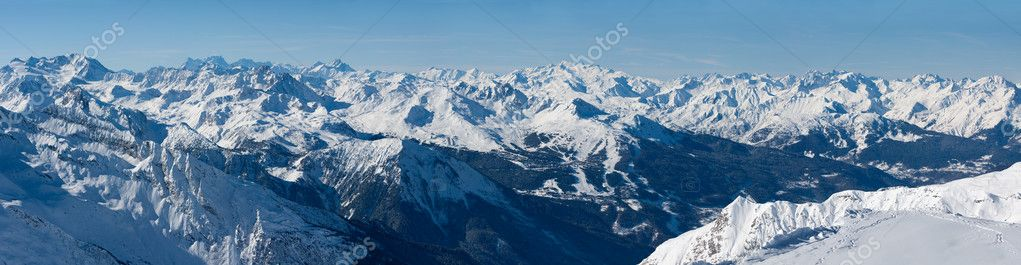
\includegraphics[width=\linewidth]{images/wide.jpeg}
    %\sidecaption[][-2.5cm]{一张宽说家罗贯中根据陈寿《三国志》和裴松之注解以图}
    \caption{一张宽说家罗贯中根据陈寿《三国志》和裴松之注解以图}
\end{figure}
\begin{figure*}
    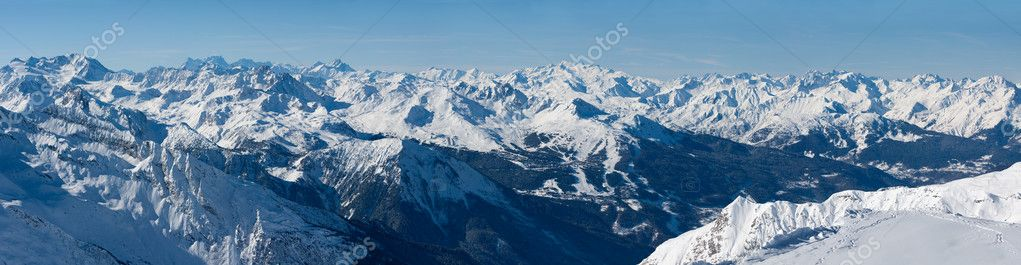
\includegraphics[width=\linewidth]{images/wide.jpeg}
    %\sidecaption[][-0.5cm]{一张宽说家罗贯中根据陈寿《三国志》和裴松之注解以图}
    \caption{一张宽说家罗贯中根据陈寿《三国志》和裴松之注解以图}
\end{figure*}
《三国演义》是\emph{罗贯中}在有关{\sffamily 三国故事的宋元话本}、戏曲和轶事传闻的基础上。依据晋代陈寿所著的《三国志》以及南朝宋人裴松之为《三国志》所作的注,所进行的加工再创作。
\begin{equation}
    \int_a^b\sin(\frac{a}{b}\sqrt{x})dx
\end{equation}

《三国演义》(全名为《三国志通俗演义》,又称《三国志演义》)(The Romance of Three Kingdoms)是元末明初小说家罗贯中根据陈寿《三国志》和裴松之注解以及民间三国故事传说经过艺术加工创作而成的长篇章回体$\frac{a}{b}$历史演义小说。与《西游记》《水浒传》《红楼梦》并称为中国古典四大名著。

《三国演义》(全名为《三国志通俗演义》,又称《三国志演义》)(The Romance of Three Kingdoms)是元末明初小说家罗贯中根据陈寿《三国志》和裴松之注解以及民间三国故事传说经过艺术加工创作而成的长篇章回体$\frac{a}{b}$历史演义小说。与《西游记》《水浒传》《红楼梦》并称为中国古典四大名著。

\begin{figure*}
    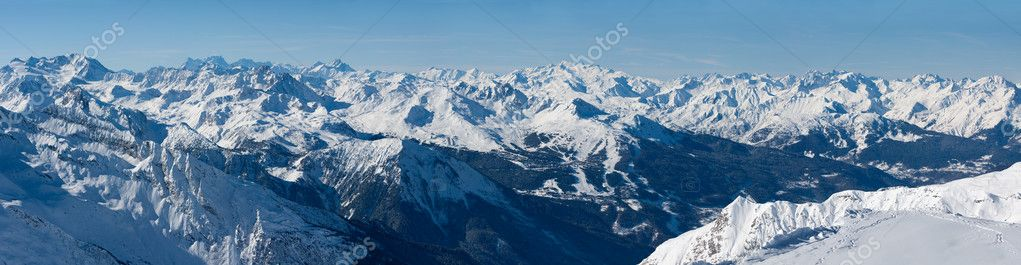
\includegraphics[width=\linewidth]{images/wide.jpeg}
    %\sidecaption[][-0.5cm]{一张宽元末明初小说家罗贯中根据陈寿《三国志》和裴松之注解图}
    \caption{一张宽图宽元末明初小说家罗贯中根据陈寿}
\end{figure*}

《三国演义》是\emph{罗贯中}在有关{\sffamily 三国故事的宋元话本}、戏曲和轶事传闻的基础上。依据晋代陈寿所著的《三国志》以及南朝宋人%
\marginnote{This article explains how to create margin notes, a popular \textbf{alternative}.}[2cm]%
裴松之为《三国志》所作的注,所进行的加工再创作。
\begin{equation}
    \int_a^b\sin(\frac{a}{b}\sqrt{x})dx
\end{equation}

\begin{equation}
    \int_a^b\sin(\frac{a}{b}\sqrt{x})dx
\end{equation}
